\documentclass[10pt,a4paper]{article}
\usepackage[utf8]{inputenc}
\usepackage{amsmath}
\usepackage{graphicx}
\usepackage{subfig}
\usepackage{amsfonts}
\setlength{\parindent}{0cm}
\usepackage{amssymb}
\author{Ferreyra Emanuel; Martin Rafael; Postolski Ivan}
\title{Modelado y simulación para un sistema controlado de dinámica SIR con Vacunación en un entorno de grafo estocástico.}
\begin{document}


\part*{Simulaci\'on de Eventos Discretos TP1}
\section*{Modelado y simulación para un sistema controlado de dinámica SIR con Vacunación en un entorno de grafo estocástico.}
\textbf{Ferreyra Emanuel; Martin Rafael; Postolski Ivan}
\vspace{3cm}

\part*{Modelo Conceptual}

Nos encargaremos de modelar una poblaci\'on de $N$ individuos que interaccionan entre s\'i, dando lugar a la propagaci\'on de una enfermedad determinada. En cada momento, los individuos pueden encontrarse en uno de los siguientes estados:
\begin{itemize}
\item Susceptible $(S)$
\item Infectado $(I)$
\item Recuperado $(R)$
\item Vacunado $(V)$
\end{itemize}


La din\'amica de infecci\'on seguir\'a las siguientes reglas:


\begin{itemize}
\item La interacci\'on entre individuos se da de a pares seg\'un un proceso aleatorio
\item Cuando un individuo Susceptible interact\'ua con uno Infectado, el primero se infecta autom\'aticamente.
\item Un individuo Infectado permanece en ese estado durante un tiempo exponencial de parametro $\rho$ despu\'es del cual pasa a estado Recuperado y ya no puede infectarse nunca mas.
\item El resto de las interaccones no modifican los estados de los individuos.
\end{itemize}


La principal diferencia con la mayor\'ia de los sistemas evolutivos de infecciones ser\'a que los individuos son racionales y podr\'an tomar la decisi\'on de vacunarse. Esto lo har\'an siguiendo una estrategia $(E)$ que puede depender del tiempo y de la proporci\'on de infectados en alg\'un subconjunto de la poblacion e indicara la tasa de vacunaci\'on.
Dicha estrategia ser\'a elegida individualmente intentando minimizar los costos asociados tanto de vacunarse como de estar infectado.


Adem\'as, las interacciones entre individuos se dan a partir de un grafo estoc\'astico construido seg\'un una distribuci\'on de grados llamado Configuration Model, donde los nodos representaran individuos y las aristas potenciales interacciones entre s\'i. Es decir que un individuo $X$ podr\'a interactuar solamente con un individuo $Y$ si existe una arista $(X,Y)$ en el grafo.


Inicialmente se definira un conjunto de individuos cuyo estado en la simulaci\'on sera Infectado a fines de modelar el inicio de la enfermedad.


RQs:
\begin{enumerate}
\item ¿C\'omo influye la distribuci\'on de grado en la propagaci\'on de la enfermedad?
\item ¿C\'omo influye la distribuci\'on de grado las estrategias de vacunaci\'on?
\item ¿C\'omo influye el conjunto inicial de indiviuos en la propagacion de la enfermedad?
\end{enumerate}




\part*{Modelo Formal}
\section*{At\'omico individuo}


Consideraremos que cada At\'omico individuo posee un $ID \in \mathbb{N}$. Adem\'as, tanto $\rho$ como $\gamma$ son par\'ametros fijos del problema, y representan las tasas de recuperaci\'on y emparejamiento/encuentro.


$Individuo=<X,Y,S,\delta_{int},\delta_{ext},\lambda,ta>$\\


$X=\{ID.1=\text{``Soy ID y me Infectaron''};ID.2=\text{``Soy ID y te infect\'e''}; \\ ID.3= \text{``Soy ID y me vacun\'e''};ID.4=\text{``Soy ID y me recuper\'e''} \}$\\


$Y=X$\\


$S=\{(estado\in\{\text{Susceptible, Pre-Infectado, Infectado, Recuperado,} \\ \text{ Vacunado}\}, ID \in \mathbb{N}, \pi \in [0,\nu], Vecinos \subset \mathbb{N}, Infectados \subseteq Vecinos, \\ Susceptibles \subseteq Vecinos\}$\\




$\delta_{ext}(s,e,ID.1)\{ \\
\hspace*{1cm} s'=s;\\
\hspace*{1cm}    s'.Infectados=s'.Infectados.add(ID);\\
\hspace*{1cm}     s'.Susceptibles=s'.Susceptibles.remove(ID);\\
\hspace*{1cm}    if\thinspace  s'.estado==Susceptible;\\
\hspace*{2cm}                    s'.\pi=\nu/s'.Vecinos.size() * s'.Infectados.size();\\
\hspace*{2cm}                    ta=exp(s'.\pi)\\
\hspace*{1cm}    if\thinspace s'.estado==Infectado;\\
\hspace*{2cm}                    ta=exp(\rho+s'.Susceptibles.size()*\gamma);\\
\hspace*{2cm}                    x=uniforme(\rho+s'.Susceptibles.size()*\gamma);\\
\hspace*{2cm}            if\thinspace x<\rho:\\
\hspace*{3cm}                            s’.recuperado=True;\\
\hspace*{2cm}                    else:\\
\hspace*{3cm}                            s’.recuperado=False;\\
\hspace*{1cm}    else:\\
\hspace*{2cm}                    ta = ta - e\\
    \}
$\\




$\delta_{ext}(s,e,ID.2)\{ \\
\hspace*{1cm}s'=s;\\
\hspace*{1cm}s'.estado = Pre-Infectado;\\
\hspace*{1cm}ta = 0;\\
    \}
$\\




$\delta_{ext}(s,e,ID.3)\{ \\
\hspace*{1cm}s'=s;\\
\hspace*{1cm}s'.Vacunados=s'.Vacunados.add(ID);\\
\hspace*{1cm}s'.Susceptibles=s'.Susceptibles.remove(ID);\\
\hspace*{1cm}if\thinspace s'.estado==Infectado;\\
\hspace*{2cm}        ta=exp(\rho+s'.Susceptibles.size()*\gamma);\\
\hspace*{1cm}else:\\
\hspace*{2cm}        ta = ta - e;\\
        \}
$\\






$\delta_{ext}(s,e,ID.4)\{ \\
\hspace*{1cm}s'=s;\\
\hspace*{1cm}s'.Infectados=s'.Infectados.remove(ID);\\
\hspace*{1cm}if\thinspace s'.estado==Susceptible;\\
\hspace*{2cm}        s'.\pi=\nu/s'.Vecinos.size() * s'.Infectados.size();\\
\hspace*{2cm}        ta=exp(s'.\pi)\\
\hspace*{1cm}else:\\
\hspace*{2cm}        ta = ta - e;\\
        \}
$\\


$\lambda(s)\{ \\
\hspace*{1cm}if\thinspace s.estado == Susceptible\\
\hspace*{2cm}        for v in s.Susceptibles.union(s.Infectados):\\
\hspace*{3cm}            send(out_v,ID.3)\\
\hspace*{1cm}if\thinspace s.estado == Pre-Infectado\\
\hspace*{2cm}        for v in s.Susceptibles:\\
\hspace*{3cm}            send(out_v,ID.1)\\
\hspace*{1cm}if\thinspace s.estado == Infectado:\\
\hspace*{2cm}   if\thinspace s.recuperado: \\
\hspace*{3cm}            for vs in s.Susceptibles:\\
\hspace*{4cm}                send(out_vs,ID.4)\\
\hspace*{1cm}        else:\\
\hspace*{2cm}            aInfectar = elijo\_uno\_uniforme(s.Susceptibles)\\
\hspace*{2cm}            send(out_aInfectar,ID.2)\\
 \}
$\\


$\delta_{int} \{\\
\hspace*{1cm}s’ = s\\
\hspace*{1cm}if\thinspace s’.estado == Susceptible:\\
\hspace*{2cm}        s’.estado = Vacunado\\
\hspace*{2cm}        ta = inf\\
\hspace*{1cm}if\thinspace s’.estado == Pre-infectado:\\
\hspace*{2cm}        s’.estado = Infectado\\
\hspace*{2cm}        x=uniforme(\rho+s'.Susceptibles.size()*\gamma);\\
\hspace*{2cm}if\thinspace x<\rho:\\
\hspace*{3cm}                s’.recuperado=True;\\
\hspace*{2cm}            else:\\
\hspace*{3cm}                s’.recuperado=False;\\
\hspace*{2cm}        ta = exp(\rho+s'.Susceptibles.size()*\gamma);\\
\hspace*{1cm}if\thinspace s’.estado == Infectado \quad \&\&\quad s’.recuperado:\\
\hspace*{2cm}        s’.estado=Recuperado;\\
\hspace*{2cm}ta = inf\\
\hspace*{1cm}if\thinspace s’.estado == Infectado \quad\&\&\quad not(s’.recuperado):\\
\hspace*{2cm}		 x=uniforme(\rho+s'.Susceptibles.size()*\gamma);\\
\hspace*{2cm}        ta = x \\
\hspace*{2cm}ta = exp(\rho+s'.Susceptibles.size()*\gamma);\\
\}
$\\


\section*{Configuration Model}


Un Configuration Model es un grafo estoc\'astico $G=<ID,{(ID,ID)}>$ definido de manera que el grado de $v \in$ ID  sigue una distribuci\'on $D$ fija.
La din\'amica de construcci\'on de este tipo de grafos es la siguiente:
\begin{enumerate}
\item A cada nodo se le asigna una cantidad de semiaristas siguiendo la distribuci\'on $D$.
\item Luego, se une al azar la semiarista de un nodo con alguna semiarista de otro nodo, tambi\'en elegida uniformemente entre las no apareadas.
\item Se repite $2$ hasta formar todas las aristas.
\end{enumerate}

Un resultado importante sobre este tipo de grafos es que para una cantidad de nodos suficientemente grande la probabilidad de que resulte ser un multigrafo, varias aristas entre dos nodos o una arista conectada a si misma, es 0. Haciendo uso de esto, el grafo base de los links entre at\'omicos estar\'a ``limpio'' de multiaristas.


\section*{Creacion de Modelo Devs}


Definimos genModelDevs: CM $\rightarrow$ DevsModel tal que:
\begin{enumerate}
\item Por cada id $\in$ CM.ID, existe un id en DevsModel.atomicos()
\item Por cada arista (x,y)  $\in$ CM.A, existen dos conexiones:
\begin{enumerate}
\item x.in.y conectado a y.out.x
\item y.in.x conectado a x.out.y
\end{enumerate}

\end{enumerate}
Bajo esta configuraci\'on, cada at\'omico individuo tendr\'a un puerto $in$ y uno $out$ por cada vecino que tenga en el grafo estoc\'astico, teniendo cuidado que el mismo n\'umero de puerto se utilice para el mismo vecino. Esto ser\'a la base de la identificaci\'on de vecinos, para que los eventos de mensajer\'ia sean consistentes y los estados se actualicen correctamente. 

\paragraph{Nota:} Dado que cada puerto tiene un numero identificador (ie, in0,...,in$n$). No ser\'a necesario en la implementaci\'on reflejar los $ID$ de cada nodo para identificar su vecino, sino que cada puerto de entrada $x$ in$x$ out$x$ se corresponde con el mismo vecino.   



\section*{Testing}


Para testear el correcto funcionamiento de los at\'omicos desarrollamos los siguientes tests pseudo-unitarios:
\subsection*{In Order}
\textbf{Configuracion inicial}:Un nodo Susceptible y un vecino Infectado con alto $\rho$ y bajo $\nu$.


\textbf{Configuracion esperada}: El nodo Susceptible debe pasar a Infectado, luego a Recuperado.


\subsection*{No Jump}
\textbf{Configuracion inicial}: Un grafo linea de tres nodos, el primer nodo Infectado y los otros dos Susceptibles.


\textbf{Configuracion esperada}: En ningun momento puede estar el tercer nodo infectado o Recuperado si el segundo esta Susceptible.


\subsection*{The Only Truth}
\textbf{Configuracion inicial}: Todos los nodos infectados.


\textbf{Configuracion esperada}: Todos los nodos recuperados.


\subsection*{No Power Here}
\textbf{Configuracion inicial}:Varios nodos Infectados, todos conectados con un nodo Vacunado/Recuperado.


\textbf{Configuracion esperada}:El Nodo debe permanecer Vacunado/Recuperado en todo momento.


\subsection*{The Spy}
\textbf{Configuracion inicial}: Dos componentes conexas de Susceptibles y un Infectado en una de ellas.


\textbf{Configuracion esperada}:Una componente con todos Recuperados o Vacunados y otra con todos Susceptibles.

\paragraph{}
Todos los comportamientos de la versión entregada se correspondieron con los esperados en los tests, validando los casos considerados interesantes. Por otro lado, como herramienta alternativa de verificación del resultado del simulador, se implementó un script llamado \textbf{sanity\_test.py} en el cual se verifica que la secuencia de estados de cada nodo sea una secuencia válida. 

\part*{Modelado y Simulaci\'on}
\section*{Resultados de la simulaci\'on}

Simulamos el modelo con $N=1000$ individuos, un porcentaje de infectados iniciales del 1\% y una distribuci\'on de grados $\Gamma(\alpha,\beta)$ con varios par\'ametros diferentes, con el fin de variar el desv\'io est\'andar aunque manteniendo constante la esperanza en 10. A continuaci\'on graficamos c\'omo evolucionaron las proporciones de la poblaci\'on en cada estado.


\begin{figure}[hbpt]
\centering
\subfloat[$\nu=10000  \; \rho= 2000$]{
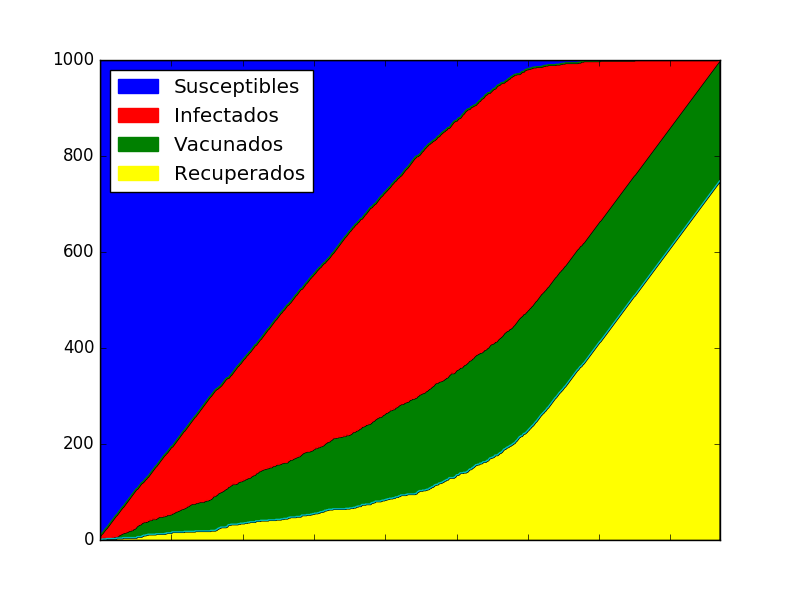
\includegraphics[scale=0.2]{gamma1000alpha30beta3log1}}
\subfloat[$\nu=1000  \; \rho= 2000$]{
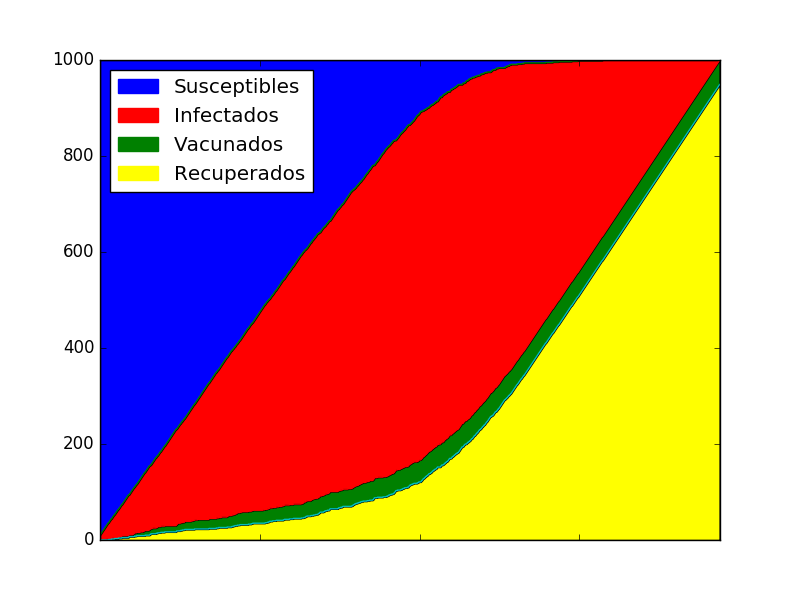
\includegraphics[scale=0.2]{gamma1000alpha30beta3log12}}
\subfloat[$\nu=100  \; \rho= 2000$]{
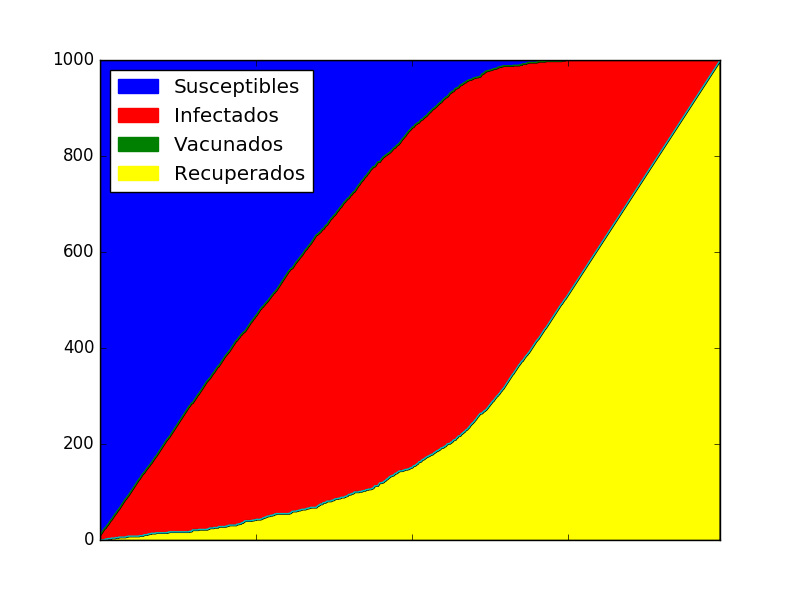
\includegraphics[scale=0.2]{gamma1000alpha30beta3log13}}
\caption{$\alpha$=30, $\beta$=3}
\end{figure}

\begin{figure}[hbpt]
\centering
\subfloat[$\nu=10000  \; \rho= 2000$]{
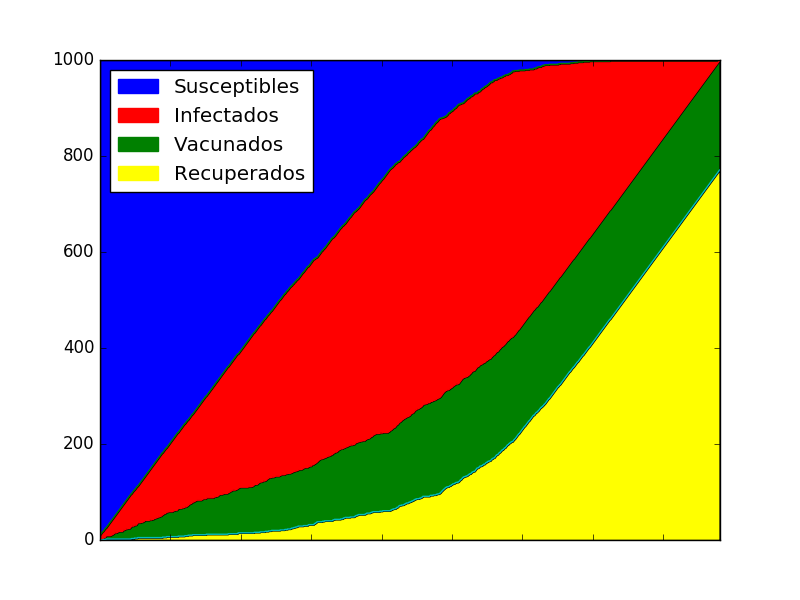
\includegraphics[scale=0.2]{gamma1000alpha3beta03log1}}
\subfloat[$\nu=1000  \; \rho= 2000$]{
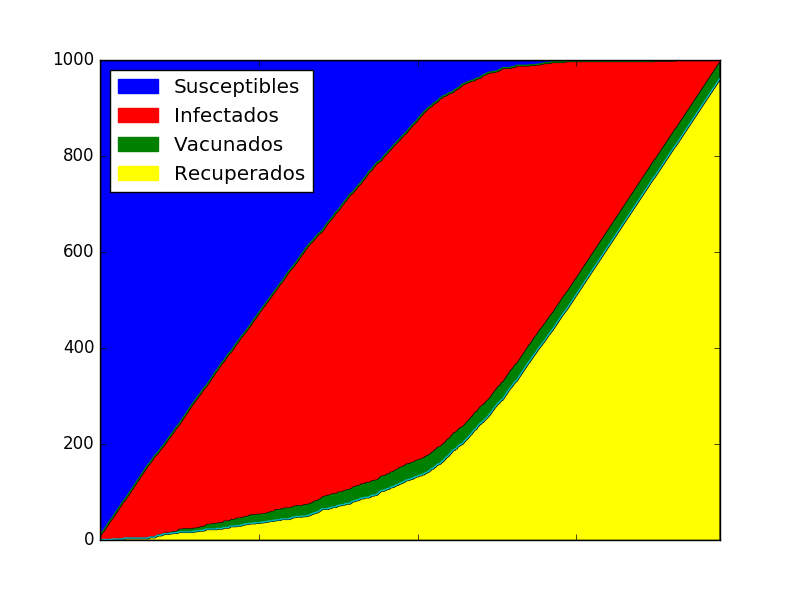
\includegraphics[scale=0.2]{gamma1000alpha3beta03log12}}
\subfloat[$\nu=100  \; \rho= 2000$]{
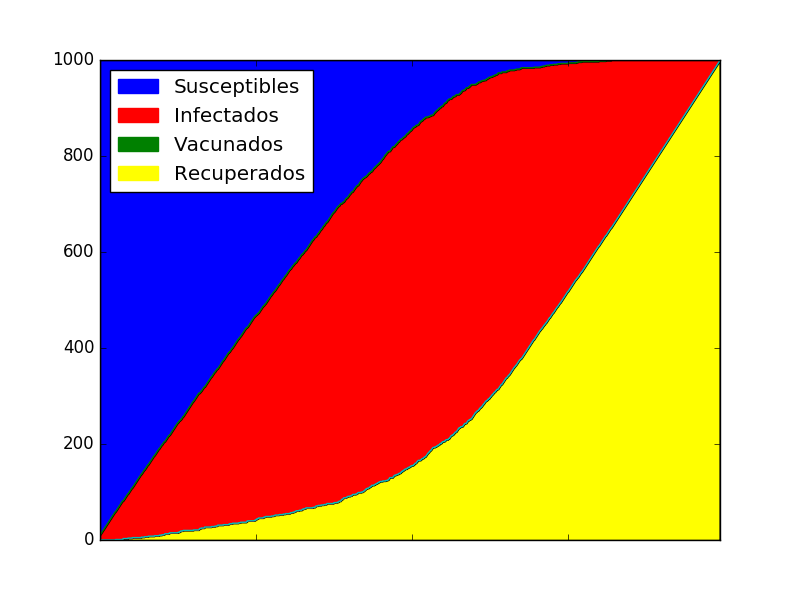
\includegraphics[scale=0.2]{gamma1000alpha3beta03log13}}
\caption{$\alpha$=3, $\beta$=0.3}
\end{figure}

\begin{figure}[hbpt]
\centering
\subfloat[$\nu=10000  \; \rho= 2000$]{
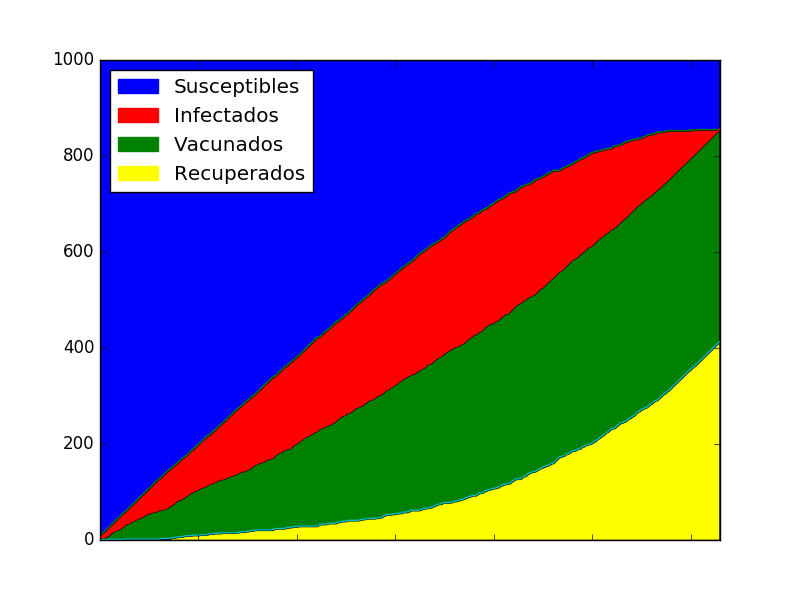
\includegraphics[scale=0.2]{gamma1000alpha1beta01log1}}
\subfloat[$\nu=1000  \; \rho= 2000$]{
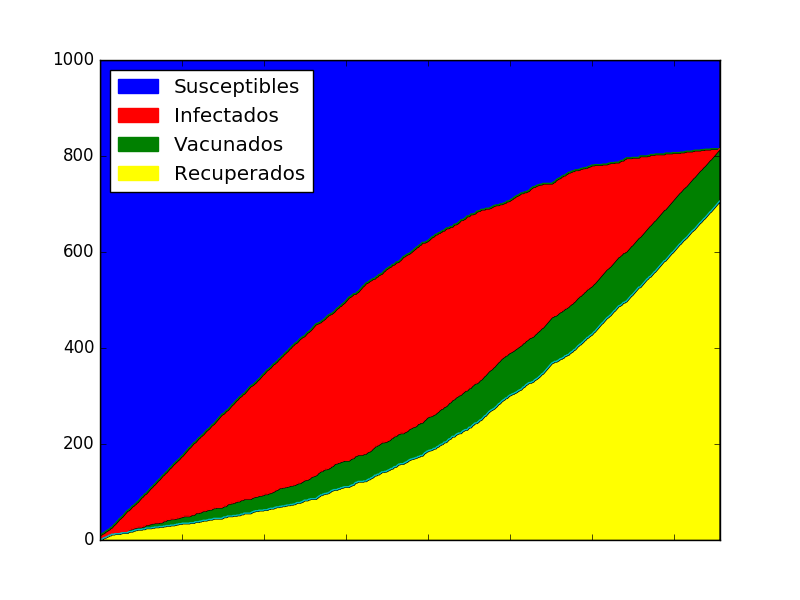
\includegraphics[scale=0.2]{gamma1000alpha1beta01log12}}
\subfloat[$\nu=100  \; \rho= 2000$]{
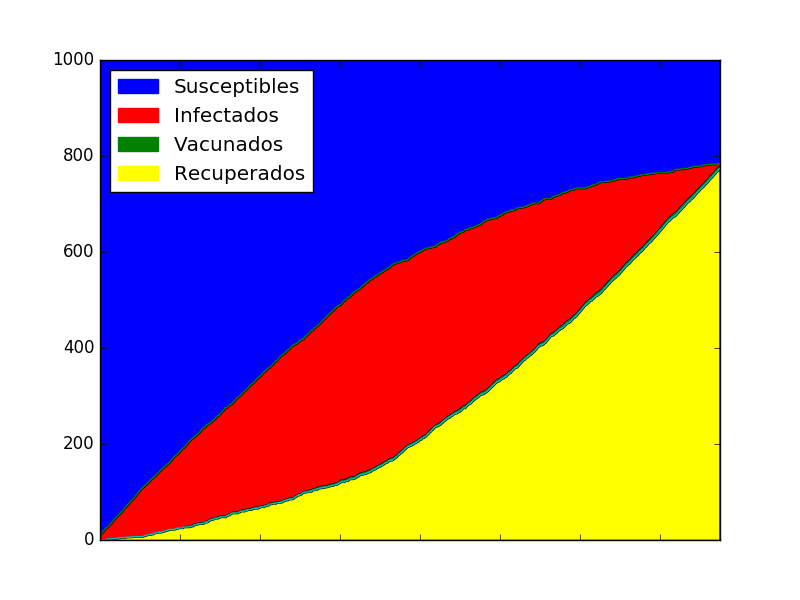
\includegraphics[scale=0.2]{gamma1000alpha1beta01log13}}
\caption{$\alpha$=1, $\beta$=0.1}
\end{figure}

\begin{figure}[hbpt]
\centering
\subfloat[$\nu=10000  \; \rho= 2000$]{
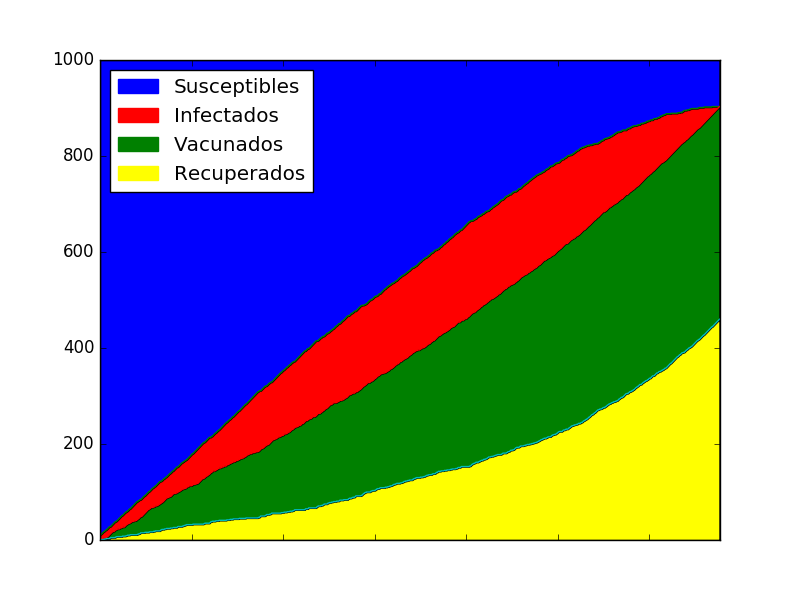
\includegraphics[scale=0.2]{gamma1000alpha10beta1log1}}
\subfloat[$\nu=1000  \; \rho= 2000$]{
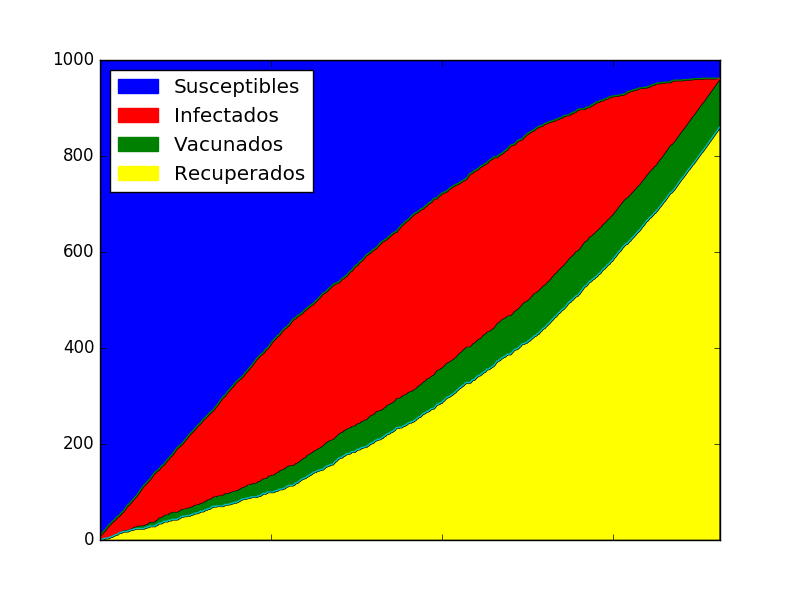
\includegraphics[scale=0.2]{gamma1000alpha10beta1log12}}
\subfloat[$\nu=100  \; \rho= 2000$]{
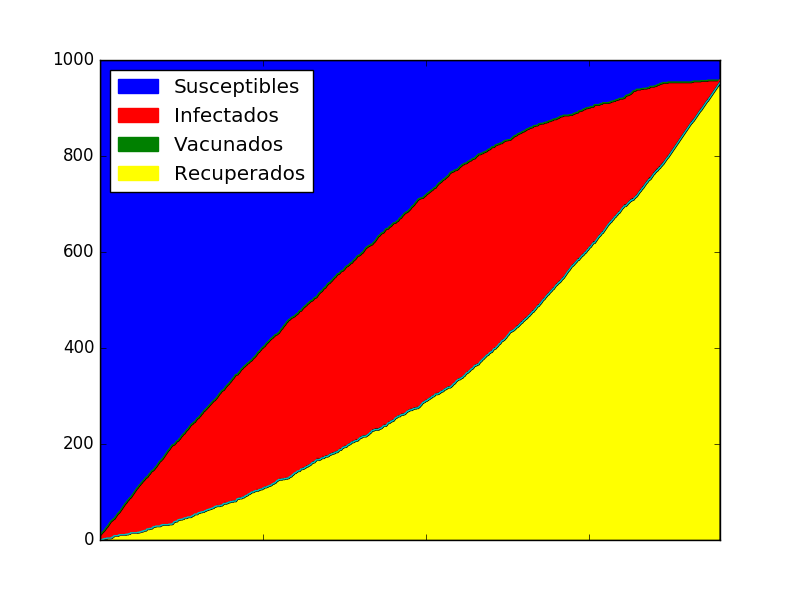
\includegraphics[scale=0.2]{gamma1000alpha10beta1log13}}
\caption{$\alpha$=10, $\beta$=1}
\end{figure}

\section*{Discusi\'on}
\paragraph{}
Podemos notar que en todos los casos el gr\'afico (a) presenta mayor proporci\'on de vacunados dado que $\nu$ es la tasa m\'axima de vacunaci\'on, que decrece en (b) y (c).

\paragraph{}
Adem\'as, tanto en la figura 1 como en la 2, la cantidad de individuos que permanece susceptible al final de la simulaci\'on es casi nula por tener menor varianza la distribuci\'on de grados. Esto hace que la enfermedad se propague m\'as r\'apidamente. El mismo fen\'omeno afecta la velocidad con la que la enfermedad se propaga, dado que los par\'ametros hacen menos probable que el grado de un nodo sea peque\~no.

\paragraph{}
El an\'alisis de la cantidad de vacunados nos indica que con este tipo de estrategias proporcionales a la cantidad de vecinos enfermos, la infecci\'on se propagar\'a, dando motivaci\'on al posterior estudio de una estrategia \'optima de vacunaci\'on, deseablemente dependiente de los grados de cada nodo y no de los infectados.




\end{document}



